\documentclass{article}
\usepackage[utf8]{inputenc}
\usepackage{graphicx}
\usepackage{hyperref}
\usepackage[nonumberlist,nopostdot]{glossaries}
\usepackage{parskip}
\setlength{\parindent}{0pt}

\title{Modern web framework in Golang}
\author{Senior design project (Spring 2016--Fall 2016)}
\date{\today}
\makeglossaries

\begin{document}

\maketitle

\section{Introduction}

Our project is to design and build a framework to improve the process of developing web applications in Golang. Golang, also referred to as Go, is an open source programming language developed at Google that emphasizes concurrency and safety. Since the language’s inception in 2009, Go has been quickly gaining popularity for use on high-performance, concurrent servers.

The web framework we will build addresses the need of web developers to quickly bootstrap and reliably maintain web applications in Go. A primary goal of the framework is to integrate with technologies such as Docker to provide first-class support for painless and rapid application deployment. The framework would provide developers a command-line \textsc{api} to generate an extensible boilerplate code to quickstart application development.

Facilitating the use of contemporary design patterns is another motivation for our web framework. Paridigms such as unidirectional data flow, function decorators, and database abstraction are popular and effective tools for web application development that our framework hopes to implement.

The project involves the challenges of architecting a large software application; routing \textsc{http} requests concurrently and securely; linking datastores, views, and controllers; and providing a unified interface for database queries. The components of the application would be tested continuously throughout the development cycle using unit tests and continuous integration (\textsc{ci}). Documentation to use the framework and an example web application built using the framework will also be included for user reference. 

\section{Web frameworks}

// TODO: overhaul

The data flow between clients and server define a web application. The Model-View-Controller (\textsc{mvc}) architecture helps programmers visualize the interactions between data components. Most user-facing web applications need to: store, persist, and retrieve user data (Model); handle and route user requests to manipulate the data (Controller); and represent information to the user in a variety of formats---\textsc{html, json}, etc. (View). The separation of duties into these categories helps isolate.

This separation facilitates web development by helping developers understand interactions between different data components. 

\subsection{Scalability and the need for frameworks in more languages}
 
Most of the popular frameworks that have emerged in the past decade are made for dynamically typed languages. They include Ruby on Rails (for the Ruby programming language), Django (for Python), and Sails.js (for JavaScript). However, large projects written in scripting languages such as Ruby, Python, and JavaScript without type-checking are unwieldy to maintain and difficult to scale, as many companies such as Twitter have discovered.\footnote{{https://blog.twitter.com/2011/the-engineering-behind-twitter-s-new-search-experience}}

As a result, more performant languages such as Java, Scala, and C\texttt{++} continue to be used by large companies for their backend infrastructures. Go is an upcoming language that belongs to this category.

\subsection{Golang MVC frameworks}

Go currently has a few third-party libraries that facilitate developing web applications---most are fairly lightweight and some follow the \textsc{mvc} paradigm. Gorilla and Martini are two popular libraries, but they make a conscious effort to be lightweight (in fact, Gorilla is just a collection of discrete packages). Beego and Revel are other Golang based \textsc{mvc} framework solutions. 

\section{Technical details}

The project will be an exercise in best practices in concurrency, \textsc{http} specifications, \textsc{rest} principles, web security, databases, web application development, writing forward-thinking \textsc{api}s, and developing as a community. Experience or familiarity in these areas is a plus. The majority of the project will be developed using the latest stable release of Go, which currently is \texttt{go1.6}. 


\subsection{Components}

% The framework will enable developers to structure their applications using the  and to write composable middleware functions---resulting in a more expressive programming style than allowed by existing frameworks like Beego or Revel.

\begin{figure}[h]
\centering
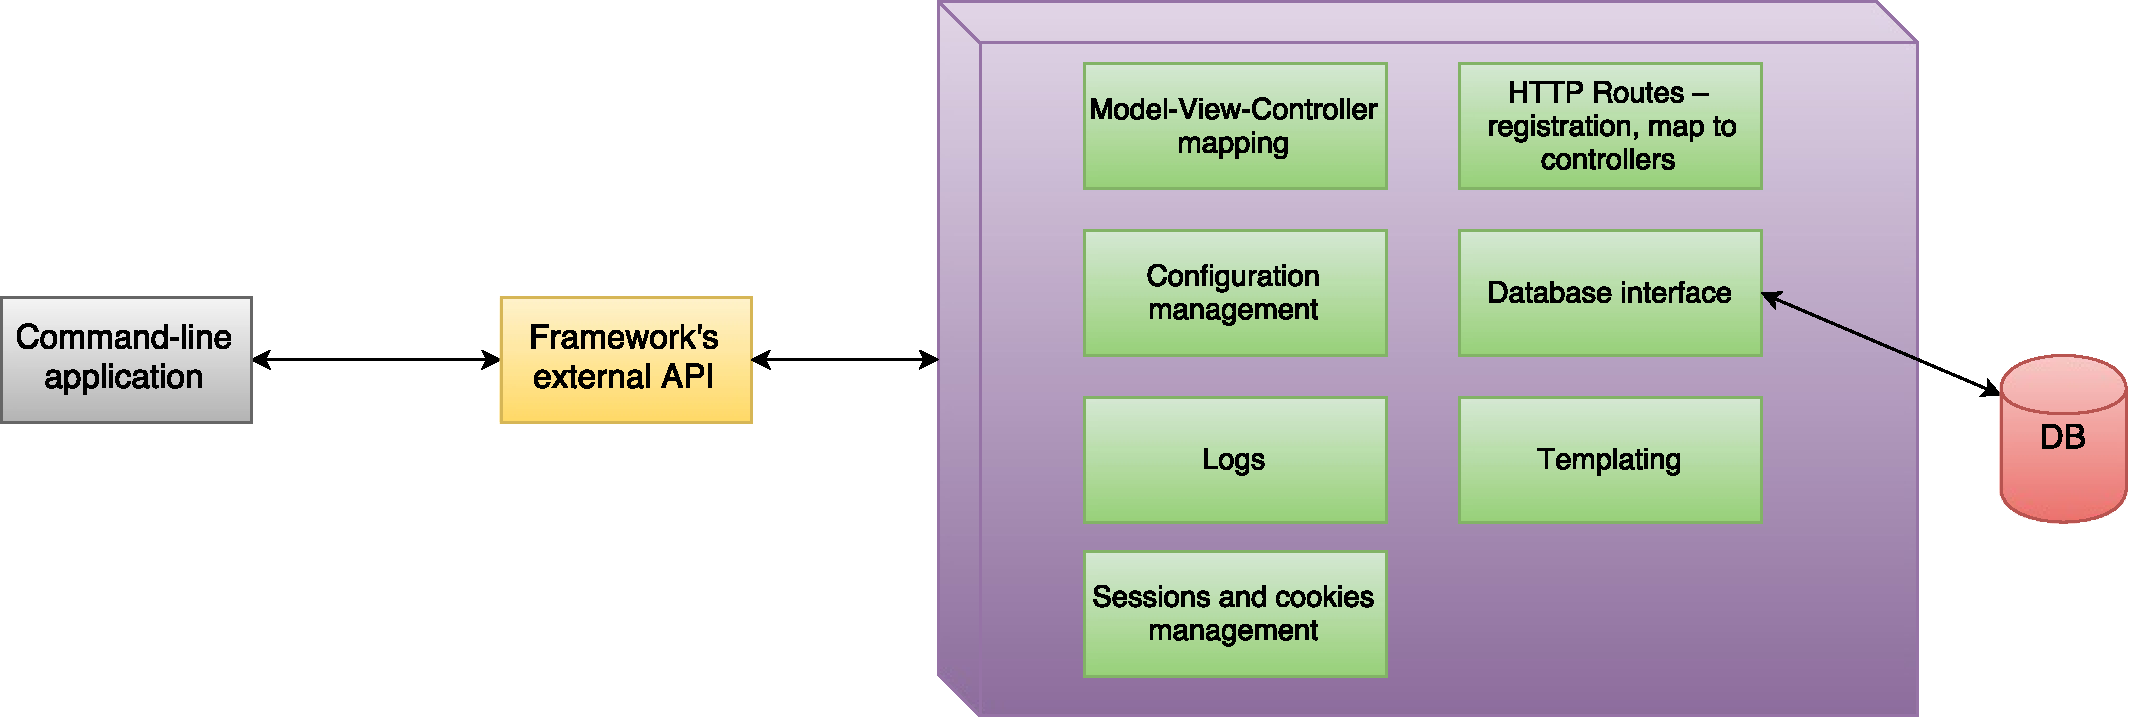
\includegraphics[width=1.1\textwidth]{mvc-app.pdf}
\caption{Major framework components }
\end{figure}

The major components of the framework are:

\begin{itemize}
    \item \textbf{The base of the framework}: This includes code for generating the file structure for the requested actions, dispatchers, reducers, datastore models, and views. It also involves the logic and rules for maintaining the relationships between these components through the lifetime of the application.
    \item \textbf{Command-line interface}: The command-line application will provide the developer access to the framework's \textsc{api}. It will allow developers to start and stop the web server; create new actions, data models, and views; configure their application; and deploy their application.
    \item \textbf{Server, router, sessions}: The framework will come with a built-in \textsc{http} server to serve applications. The plan is to make components easily swappable, so developers can choose to drop in their own \textsc{http} server, mux, or router implementation during production if needed. This would rely on Go's \texttt{net/http} package or on faster alternatives such as \texttt{valyala/fasthttp}.\footnote{The open source package available at {https://github.com/valyala/fasthttp} claims to be up to 10x faster than the built-in http package} The other related components include the router and a cookies and sessions manager. 
    \item \textbf{Database interface}: Models will need to persist on disk. Developing a domain specific query language (\textsc{dsl}) will abstract away the details of the underlying database from application developers. The interface will provide a unified way of accessing the database and make it possible to replace the underlying database safely without significant developer effort.
    \item \textbf{Templating engine}: This is required to render model data on \textsc{html} views. As of now, Go's \texttt{html/template} package appears to be a good choice---providing a good balance of performance, familiarity to users, and support for expressive programming logic directly in the view templates.
\end{itemize}

\vspace{1em}

\begin{figure}[h]
\centering
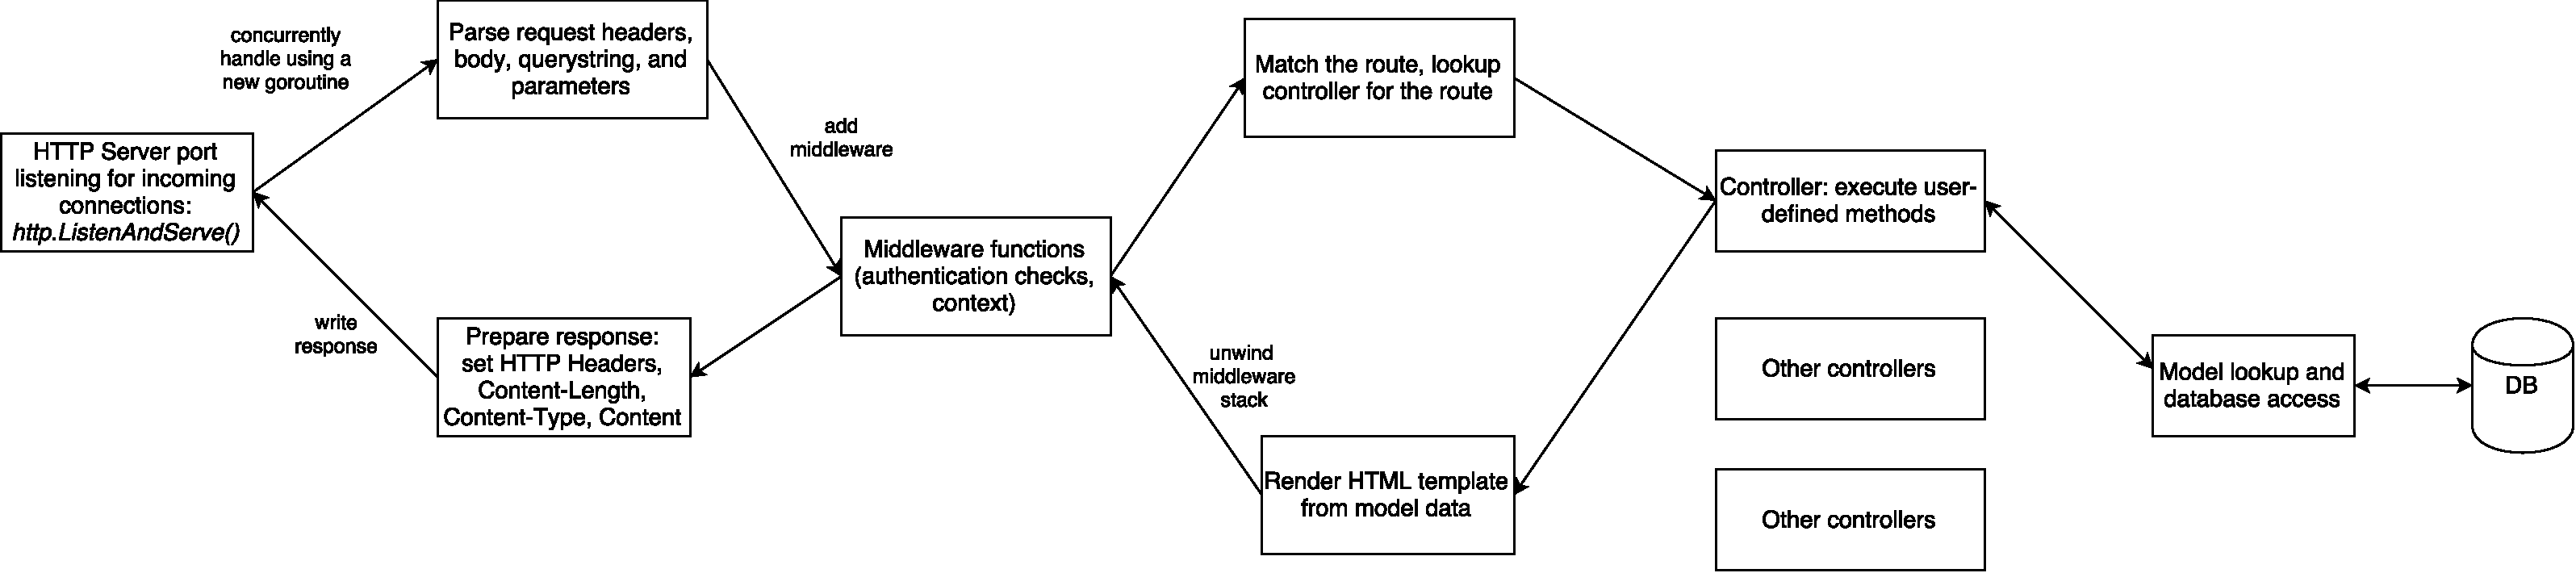
\includegraphics[width=1.1\textwidth]{mvc-run.pdf}
\caption{Framework runtime: handling a simple request}
\end{figure}

\subsection{Features}

The framework will have the following features:

\begin{itemize}
	\item Pre-configured sane default values that make it easy for developers to get a basic application running quickly.
	\item One-click/one-command deployment to Docker and container management with Kubernetes.
    \item Deployment to Heroku, Digital Ocean, and Amazon Web Services.
    \item Support for the decorator pattern and middleware functions, similar to Koa.js.
    \item Improved support for popular in-memory datastores such as Redis.
	\item Support third-party online data persistence solutions such as Firebase, Google Cloud DataStore, and AppEngine DataStore.
    \item Built-in authentication with common log-in providers such as Google, Gravatar, Twitter, and GitHub (undecided).
    \item Testing and load generation tools.
\end{itemize}

\subsection{Lines of code}

The team anticipates that the project will require around 20,000--25,000 lines of code.

\subsection{Testing}

Code coverage is an important component of the project. Unit tests will be written when appropriate. The code repositories are currently configured to use Wercker, a continuous integration and build system service, to trigger builds and tests on each commit. Testing frameworks will be added as necessary. Currently, ginkgo---a BDD testing framework---is the primary candidate.

\section{Challenges}

From initial discussions, the team currently expects these challenges:

\begin{itemize}
    \item \textbf{Architecting the framework}: The framework comprises of several distinct components which would need to be developed in parallel and integrated. The framework would need to be architected in a manner that is maintainable and flexible enough to modify on the long term.
    \item \textbf{Connecting related actions, data, views}: Naming conventions (à la Rails style) or developer configurable options should exist for mapping relations between routes, actions, data, and views. The pros and cons of either approach need to be evaluated. The implementation would need to be error- and ambiguity-free, as this is a part of the framework's logic that will be used on every incoming request for standard applications.
    \item \textbf{Internalizing the Flux pattern}: The team currently has limited familiarity with the Flux patterns. Members will need to orient themselves with basic conventions of the pattern before architecting the framework.
\end{itemize}

Thoughtful design decisions in the initial stages are important for the success of the project. Research on the beneficial parts of and criticism on existing \textsc{mvc} frameworks (including those written in other languages), and careful problem scoping should address most issues. The team would also need to spend time to get acquainted with the Go programming language.

\section{Costs}

The team does not anticipate major financial costs in the development of the framework. 

\section{Conclusion}

The team is currently in the design phase---researching existing designs, evaluating prospective tools, and formulating the architecture for the framework. Feedback and suggestions are always welcome.\\


Contact for questions, comments regarding this proposal: 

\begin{itemize}
    \item Joshua Dong $\langle jdong42@gmail.com \rangle$
    \item Brad Gray $\langle bpgray@utexas.edu \rangle$
    \item *Rahul Jaisimha $\langle rahul@jaisimha.com \rangle$


\item Salim Memon $\langle salim.memon@utexas.edu  \rangle$
    \item *Taiyi Ouyang $\langle taiyi.o@utexas.edu \rangle$
    \item *Nishanth Shanmugham $\langle nishanths@utexas.edu \rangle$
\end{itemize}

Students marked with * are honors students.

% Glossary
\newglossaryentry{api}
{
  name=API,
  description={
    Application Programming Interface. Defines an interface that software programs can use to interact
  }
}

\newglossaryentry{mvc}
{
  name=MVC,
  description={
    Model View Controller. A design paradigm in software engineering. Popular for the design of web applications.
  }
}

\newglossaryentry{ci}
{
  name=CI,
  description={
    Continuous Integration. A software development strategy in which code that is committed is tested and integrated using automation tools to catch errors early.
  }
}

\newglossaryentry{http}
{
  name=HTTP,
  description={
    Hypertext Transfer Protocol. The network protocol that is the basis of communication on the World Wide Web.
  }
}

\newglossaryentry{rest}
{
  name=REST,
  description={
    Representational State Transfer. An architectural style for web application design and resource handling. RESTful systems emphasize statelessness and generally communicate over HTTP.
  }
}

\newglossaryentry{rails}
{
  name=Rails,
  description={
    Ruby on Rails, or Rails for short, is an MVC web development framework for the Ruby programming language.
  }
}

\newglossaryentry{digitalocean}
{
  name=Digital Ocean,
  description={
    A cloud services infrastructure provider.
  }
}

\newglossaryentry{firebase}
{
  name=Firebase,
  description={
    An online, easy-to-configure database service company.
  }
}

\newglossaryentry{redis}
{
  name=Redis,
  description={
    A high-performance, in-memory data structure store commonly used for caching. 
  }
}

\newglossaryentry{appengine}
{
  name=AppEngine,
  description={
    A web application hosting platform from Google
  }
} 

\newglossaryentry{heroku}
{
  name=Heroku,
  description={
    A web application hosting company.
  }
}


\newglossaryentry{docker}
{
  name=Docker,
  description={
    Open source framework for packaging, distributing, and deploying applications.
  }
}

\newglossaryentry{kubernetes}
{
  name=Kubernetes,
  description={
    Open source software for managing containerized applications such as those running on Docker.
  }
}

\newglossaryentry{koajs}
{
  name=Koa.js,
  description={
    A JavaScript web framework that places emphasis on the use of middleware functions.
 } 
}

\glsaddall
\printglossaries

\end{document}
